\documentclass[14pt,a4paper]{extarticle}
% =============================================================
% preamble_compact.tex — компактный вариант оформления отчётов
% Основа — preamble.tex (СТП БГУИР); здесь только уплотнение:
% разделы без принудительного перехода на новую страницу,
% меньшие вертикальные отступы, плотные списки и подписи.
% =============================================================
% =============================================================
% preamble.tex — Shared LaTeX preamble for genetic/evolutionary reports
% Conforming to BSUIR STP 01-2024
% =============================================================

% Encoding and language
\usepackage[utf8]{inputenc}
\usepackage[T2A]{fontenc}
\usepackage[russian]{babel}

% Times New Roman font
\usepackage{tempora}

% Page geometry: STP 2.1.1
\usepackage{geometry}
\geometry{left=30mm, right=15mm, top=20mm, bottom=20mm}

% Line spacing: STP 2.1.1
\usepackage{setspace}
\singlespacing

% Allow TeX a bit more flexibility to avoid overflow
\pretolerance=1000
\tolerance=2000
\emergencystretch=3em

% Paragraph indent
\usepackage{indentfirst}
\setlength{\parindent}{1.25cm}

% Page numbers
\usepackage{fancyhdr}
\pagestyle{fancy}
\fancyhf{}
\fancyfoot[R]{\thepage}
\renewcommand{\headrulewidth}{0pt}
\fancypagestyle{plain}{%
  \fancyhf{}%
  \fancyfoot[R]{\thepage}%
  \renewcommand{\headrulewidth}{0pt}%
}

% Math
\usepackage{amsmath,amssymb}

% Graphics
\usepackage{graphicx}
\usepackage{float}
\usepackage{xcolor}

% Tables
\usepackage{booktabs}
\usepackage{tabularx}
\usepackage{multirow}
\usepackage{longtable}

% Captions
\usepackage{caption}
\captionsetup[figure]{
  labelsep=endash,
  justification=centering,
  font={normalsize},
  name=Рисунок
}
\captionsetup[table]{
  labelsep=endash,
  justification=raggedright,
  singlelinecheck=false,
  font={normalsize},
  name=Таблица
}

% Section formatting
\usepackage{titlesec}
\titleformat{\section}
  {\newpage\normalfont\fontsize{14}{18}\selectfont\bfseries}
  {\thesection}{0.5em}{\MakeUppercase}
\titlespacing*{\section}{1.25cm}{0pt}{14pt}

\titleformat{\subsection}
  {\normalfont\fontsize{14}{18}\selectfont\bfseries}
  {\thesubsection}{0.5em}{}
\titlespacing*{\subsection}{1.25cm}{14pt}{14pt}

\titleformat{\subsubsection}
  {\normalfont\fontsize{14}{18}\selectfont\bfseries}
  {\thesubsubsection}{0.5em}{}
\titlespacing*{\subsubsection}{1.25cm}{14pt}{14pt}

% Unnumbered sections
\newcommand{\sectioncenter}[1]{%
  \newpage
  \phantomsection
  \addcontentsline{toc}{section}{#1}
  \begin{center}
    \textbf{\MakeUppercase{#1}}
  \end{center}
  \vspace{14pt}
}

% Table of contents formatting
\usepackage{tocloft}
\renewcommand{\cftsecfont}{\normalfont}
\renewcommand{\cftsecpagefont}{\normalfont}
\renewcommand{\cftsubsecfont}{\normalfont}
\renewcommand{\cftsubsecpagefont}{\normalfont}
\renewcommand{\cftsecleader}{\cftdotfill{\cftdotsep}}
\renewcommand{\cftdotsep}{1}
\renewcommand{\contentsname}{\hfill\textbf{СОДЕРЖАНИЕ}\hfill}
\renewcommand{\cftaftertoctitle}{\hfill}

% Lists
\usepackage{enumitem}
\setlist[itemize]{noitemsep, topsep=0pt, leftmargin=1.25cm, label=--}
\setlist[enumerate]{noitemsep, topsep=0pt, leftmargin=1.25cm}

% Code listings
\usepackage{listings}
\usepackage{fancyvrb}
\lstset{
  basicstyle=\ttfamily\small,
  frame=single,
  breaklines=true,
  showstringspaces=false,
  inputencoding=utf8,
  extendedchars=true,
  literate={а}{{\cyra}}1 {б}{{\cyrb}}1 {в}{{\cyrv}}1 {г}{{\cyrg}}1
           {д}{{\cyrd}}1 {е}{{\cyre}}1 {ж}{{\cyrzh}}1 {з}{{\cyrz}}1
           {и}{{\cyri}}1 {й}{{\cyrishrt}}1 {к}{{\cyrk}}1 {л}{{\cyrl}}1
           {м}{{\cyrm}}1 {н}{{\cyrn}}1 {о}{{\cyro}}1 {п}{{\cyrp}}1
           {р}{{\cyrr}}1 {с}{{\cyrs}}1 {т}{{\cyrt}}1 {у}{{\cyru}}1
           {ф}{{\cyrf}}1 {х}{{\cyrh}}1 {ц}{{\cyrc}}1 {ч}{{\cyrch}}1
           {ш}{{\cyrsh}}1 {щ}{{\cyrshch}}1 {ъ}{{\cyrhrdsn}}1
           {ы}{{\cyrery}}1 {ь}{{\cyrsftsn}}1 {э}{{\cyrerev}}1
           {ю}{{\cyryu}}1 {я}{{\cyrya}}1
}

% Hyperlinks
\usepackage{hyperref}
\hypersetup{
  colorlinks=true,
  linkcolor=black,
  urlcolor=blue,
  citecolor=black,
}

% Number figures and tables within sections
\numberwithin{figure}{section}
\numberwithin{table}{section}
\numberwithin{equation}{section}

% Standard title page macro
\newcommand{\makegeclabtitle}[2]{%
  \begin{titlepage}
  \thispagestyle{empty}
  \begin{center}

  МИНИСТЕРСТВО ОБРАЗОВАНИЯ РЕСПУБЛИКИ БЕЛАРУСЬ

  \vspace{0.5em}

  Учреждение образования

  \vspace{0.5em}

  \textbf{<<Белорусский государственный университет информатики и радиоэлектроники>>}

  \vspace{2em}

  Факультет компьютерных систем и сетей

  \vspace{0.5em}

  Кафедра программного обеспечения информационных технологий

  \end{center}

  \vspace{3em}

  \begin{center}
  \textbf{ОТЧЕТ}

  \vspace{0.5em}

  по лабораторной работе №#1

  \vspace{0.5em}

  по дисциплине

  \vspace{0.5em}

  <<Генетические и эволюционные вычисления>>

  \vspace{0.5em}

  <<#2>>
  \end{center}

  \vspace{5em}

  \begin{flushright}
  \begin{minipage}{0.5\textwidth}
  \textbf{Выполнил:}\\
  Лебедевич Артем Владимирович\\
  магистрант группы 556301

  \vspace{0.6em}

  \textbf{Преподаватель:}\\
  Нестеренков Сергей Николаевич\\
  кандидат технических наук\\
  доцент кафедры ПОИТ
  \end{minipage}
  \end{flushright}

  \vfill

  \begin{center}
  Минск, 2026~г.
  \end{center}

  \end{titlepage}
}


% Разделы идут подряд, без \newpage
\titleformat{\section}
  {\normalfont\fontsize{14}{17}\selectfont\bfseries}
  {\thesection}{0.5em}{\MakeUppercase}
\titlespacing*{\section}{1.25cm}{12pt}{6pt}
\titlespacing*{\subsection}{1.25cm}{8pt}{4pt}

% Плотнее плавающие объекты и подписи
\setlength{\textfloatsep}{8pt plus 2pt minus 2pt}
\setlength{\floatsep}{6pt plus 2pt minus 2pt}
\setlength{\intextsep}{6pt plus 2pt minus 2pt}
\captionsetup[figure]{skip=3pt, font={small}}
\captionsetup[table]{skip=2pt, font={small}}
\setlength{\abovedisplayskip}{4pt}
\setlength{\belowdisplayskip}{4pt}

% Таблицы компактнее
\renewcommand{\arraystretch}{1.05}
\setlength{\tabcolsep}{5pt}

% Номера рисунков и таблиц — сквозные (без привязки к разделам)
\counterwithout{figure}{section}
\counterwithout{table}{section}
\counterwithout{equation}{section}

\graphicspath{{figures/}}

\begin{document}

\makegeclabtitle{6}{Поиск экстремума функции двух переменных с помощью генетического алгоритма с бинарным представлением особей}

\section{Цель работы}

Модифицировать классический генетический алгоритм с бинарным представлением для поиска экстремума функции двух переменных; изучить бинарное кодирование нескольких переменных, однородный кроссинговер, оператор инверсии и стратегии сокращения популяции. Вариант~3: минимум 7-й функции Шаффера
\begin{equation}
f(x_1, x_2) = (x_1^2 + x_2^2)^{0{,}25}\bigl[\sin^2\bigl(50\,(x_1^2 + x_2^2)^{0{,}1}\bigr) + 1\bigr], \quad x_i \in [-100;\ 100],
\end{equation}
глобальный минимум $f(0, 0) = 0$. Минимумы функции лежат концентрическими кольцами, которые сгущаются к началу координат (рисунок~\ref{fig:pop}).

\section{Краткие теоретические сведения}

\textbf{Кодирование.} Хромосома~--- конкатенация двух строк по $L$ бит; $x_i = a + \mathrm{dec}(s_i)(b - a)/(2^L - 1)$. При $L = 20$ шаг сетки $\Delta = 1{,}9 \cdot 10^{-4}$.

\textbf{Операторы.} Турнирная селекция: из $k$ случайных особей родителем становится лучшая. Однородный кроссинговер: каждый бит потомка берётся от одного из родителей по случайной маске. Инверсия: случайный отрезок хромосомы переворачивается~--- порядок битов меняется, а их состав сохраняется. Побитовая мутация инвертирует каждый бит с вероятностью $1/2L$.

\textbf{Стратегии сокращения.} Элитарная ($\mu + \lambda$): из объединения родителей и потомков остаются $N$ лучших. Чистая замена: родители полностью заменяются потомками. Случайная замена: $N$ особей выбираются из объединения случайно.

\section{Ход работы}

\textbf{Предел точности.} Точка 0 не представима 20-битным кодом: $(2^{20} - 1)/2$~--- не целое, и ближайшие узлы сетки дают $x_i = \pm\Delta/2$. Минимум $f$ по узлам сетки у начала координат равен $0{,}0200$~--- меньшего значения не получит никакой алгоритм с таким кодированием. Поэтому запуск считается успешным при $f < 0{,}1$; дополнительно фиксируется доля запусков, достигших предела $0{,}0200$, и скорость~--- поколение, на котором впервые получено $f < 0{,}1$.

\textbf{Реализация и основной запуск.} ГА реализован на NumPy (\texttt{lab\_06.ipynb}): $N = 80$, $P_c = 0{,}85$, инверсия с $P_{inv} = 0{,}2$ и побитовая мутация, турнир $k = 3$, элитарное сокращение. Результат приведён в таблице~\ref{tab:result}, динамика популяции~--- на рисунке~\ref{fig:pop}.

\begin{table}[H]
\caption{Результат основного запуска (N = 80, 300 поколений, инверсия и побитовая мутация, элитарное сокращение)}
\label{tab:result}
\centering
\small
\begin{tabular}{lc}
\toprule
Показатель & Значение \\
\midrule
Лучшая точка $(x_1; x_2)$ & (-9.54e-05; +9.54e-05) \\
Расстояние до $(0; 0)$ & 1.3e-04 \\
Лучшее $f$ (ГА) & 0.0200 \\
Нижняя граница сетки 20 бит & 0.0200 \\
Вычислений функции & 24080 \\
\bottomrule
\end{tabular}
\end{table}


\begin{figure}[H]
\centering
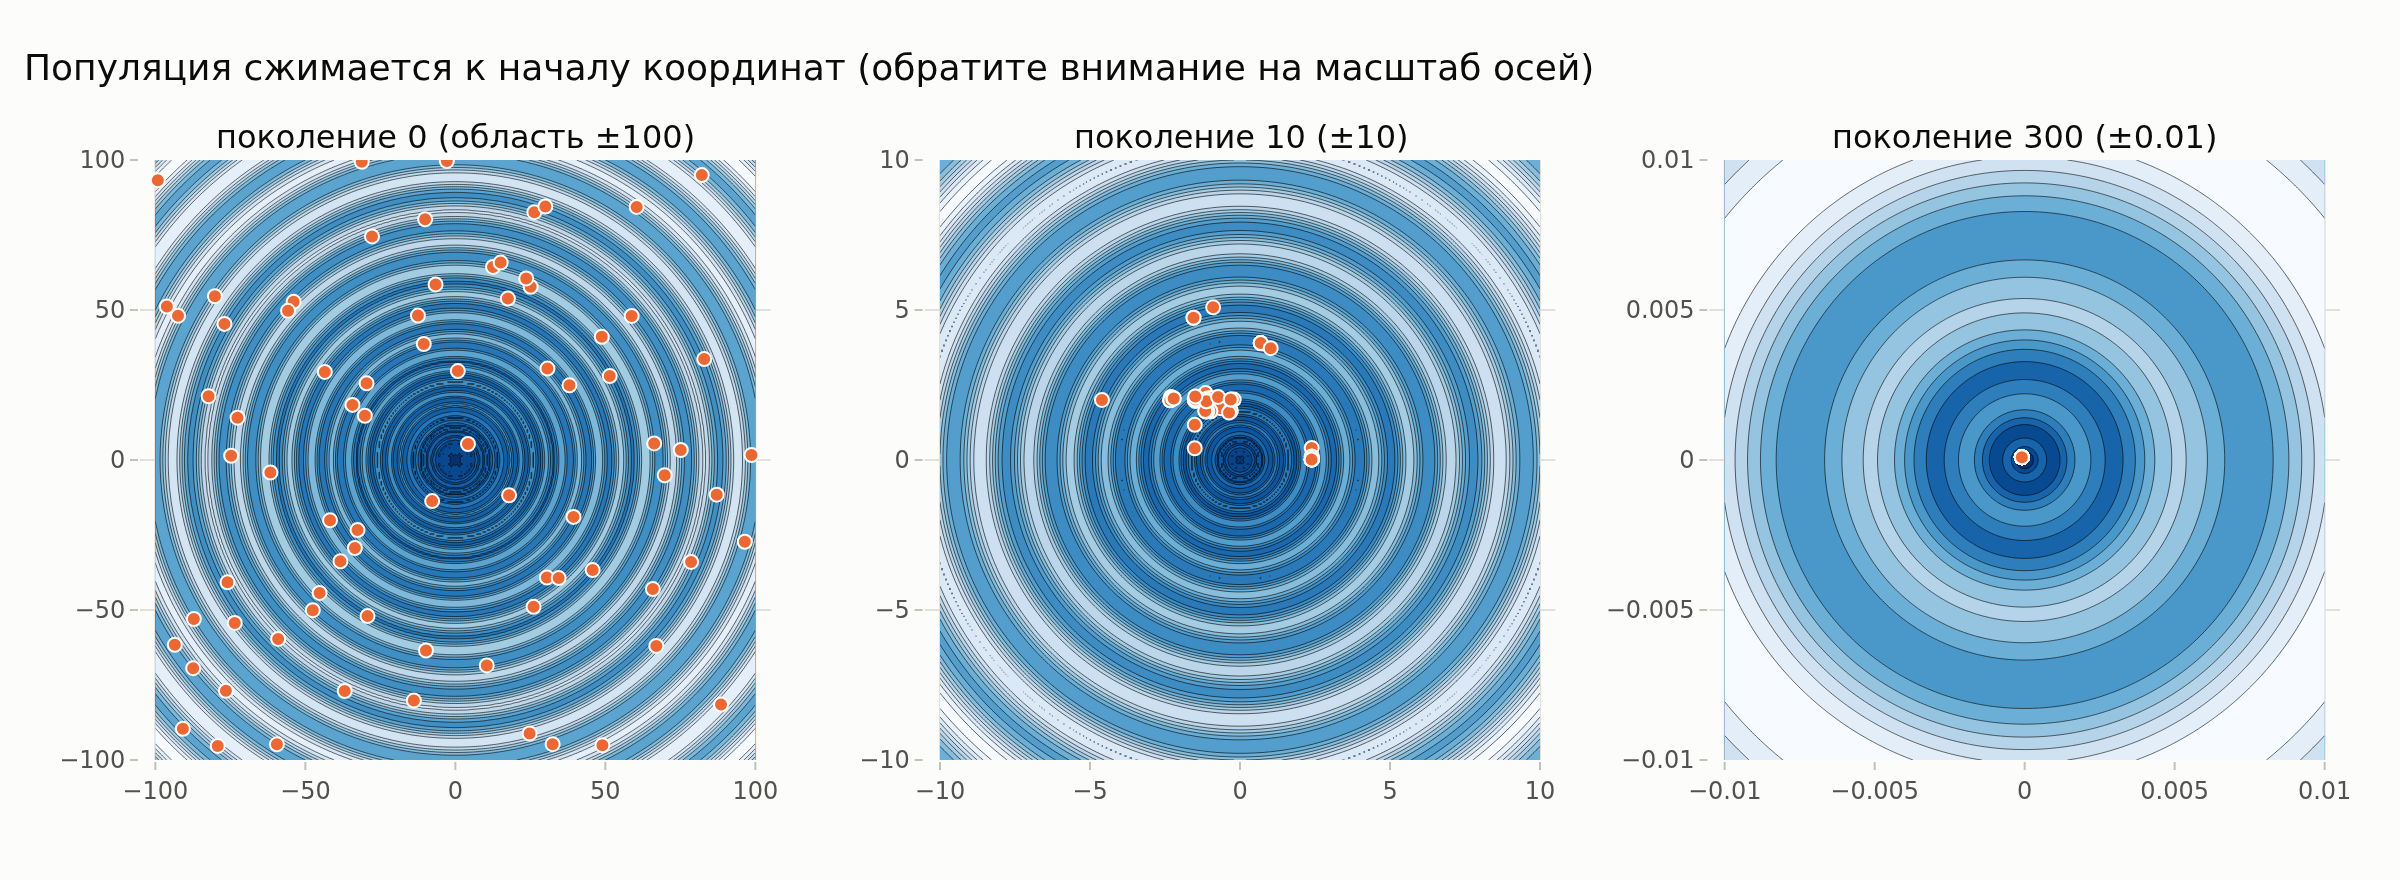
\includegraphics[width=\textwidth]{03_population.png}
\caption{Популяция на линиях уровня функции: поколения 0, 10 и 300 (масштаб осей уменьшается)}
\label{fig:pop}
\end{figure}

\textbf{Операторы мутации и стратегии сокращения.} Каждая конфигурация запускалась 20 раз (таблицы~\ref{tab:mutation}, \ref{tab:reduction}, рисунок~\ref{fig:red}).

\begin{table}[H]
\caption{Вклад операторов мутации (20 запусков, элитарное сокращение)}
\label{tab:mutation}
\centering
\small
\begin{tabular}{lccccc}
\toprule
Оператор & Медиана $f$ & Худшее $f$ & Успехов, \% & До предела, \% & Поколений \\
\midrule
инверсия + побитовая & 0.0200 & 0.031 & 100 & 90 & 26 \\
только инверсия & 0.0638 & 0.397 & 70 & 10 & 47 \\
только побитовая & 0.0200 & 0.055 & 100 & 80 & 29 \\
без мутации & 1.0128 & 2.246 & 5 & 0 & 11 \\
\bottomrule
\end{tabular}
\end{table}

\begin{table}[H]
\caption{Стратегии сокращения популяции (20 запусков)}
\label{tab:reduction}
\centering
\small
\begin{tabular}{lccccc}
\toprule
Стратегия & Медиана $f$ & Худшее $f$ & Успехов, \% & До предела, \% & Поколений \\
\midrule
элитарное ($\mu+\lambda$) & 0.0200 & 0.031 & 100 & 90 & 26 \\
чистая замена & 0.0200 & 0.021 & 100 & 65 & 44 \\
случайная замена & 0.0208 & 0.059 & 100 & 35 & 84 \\
\bottomrule
\end{tabular}
\end{table}


\begin{figure}[H]
\centering
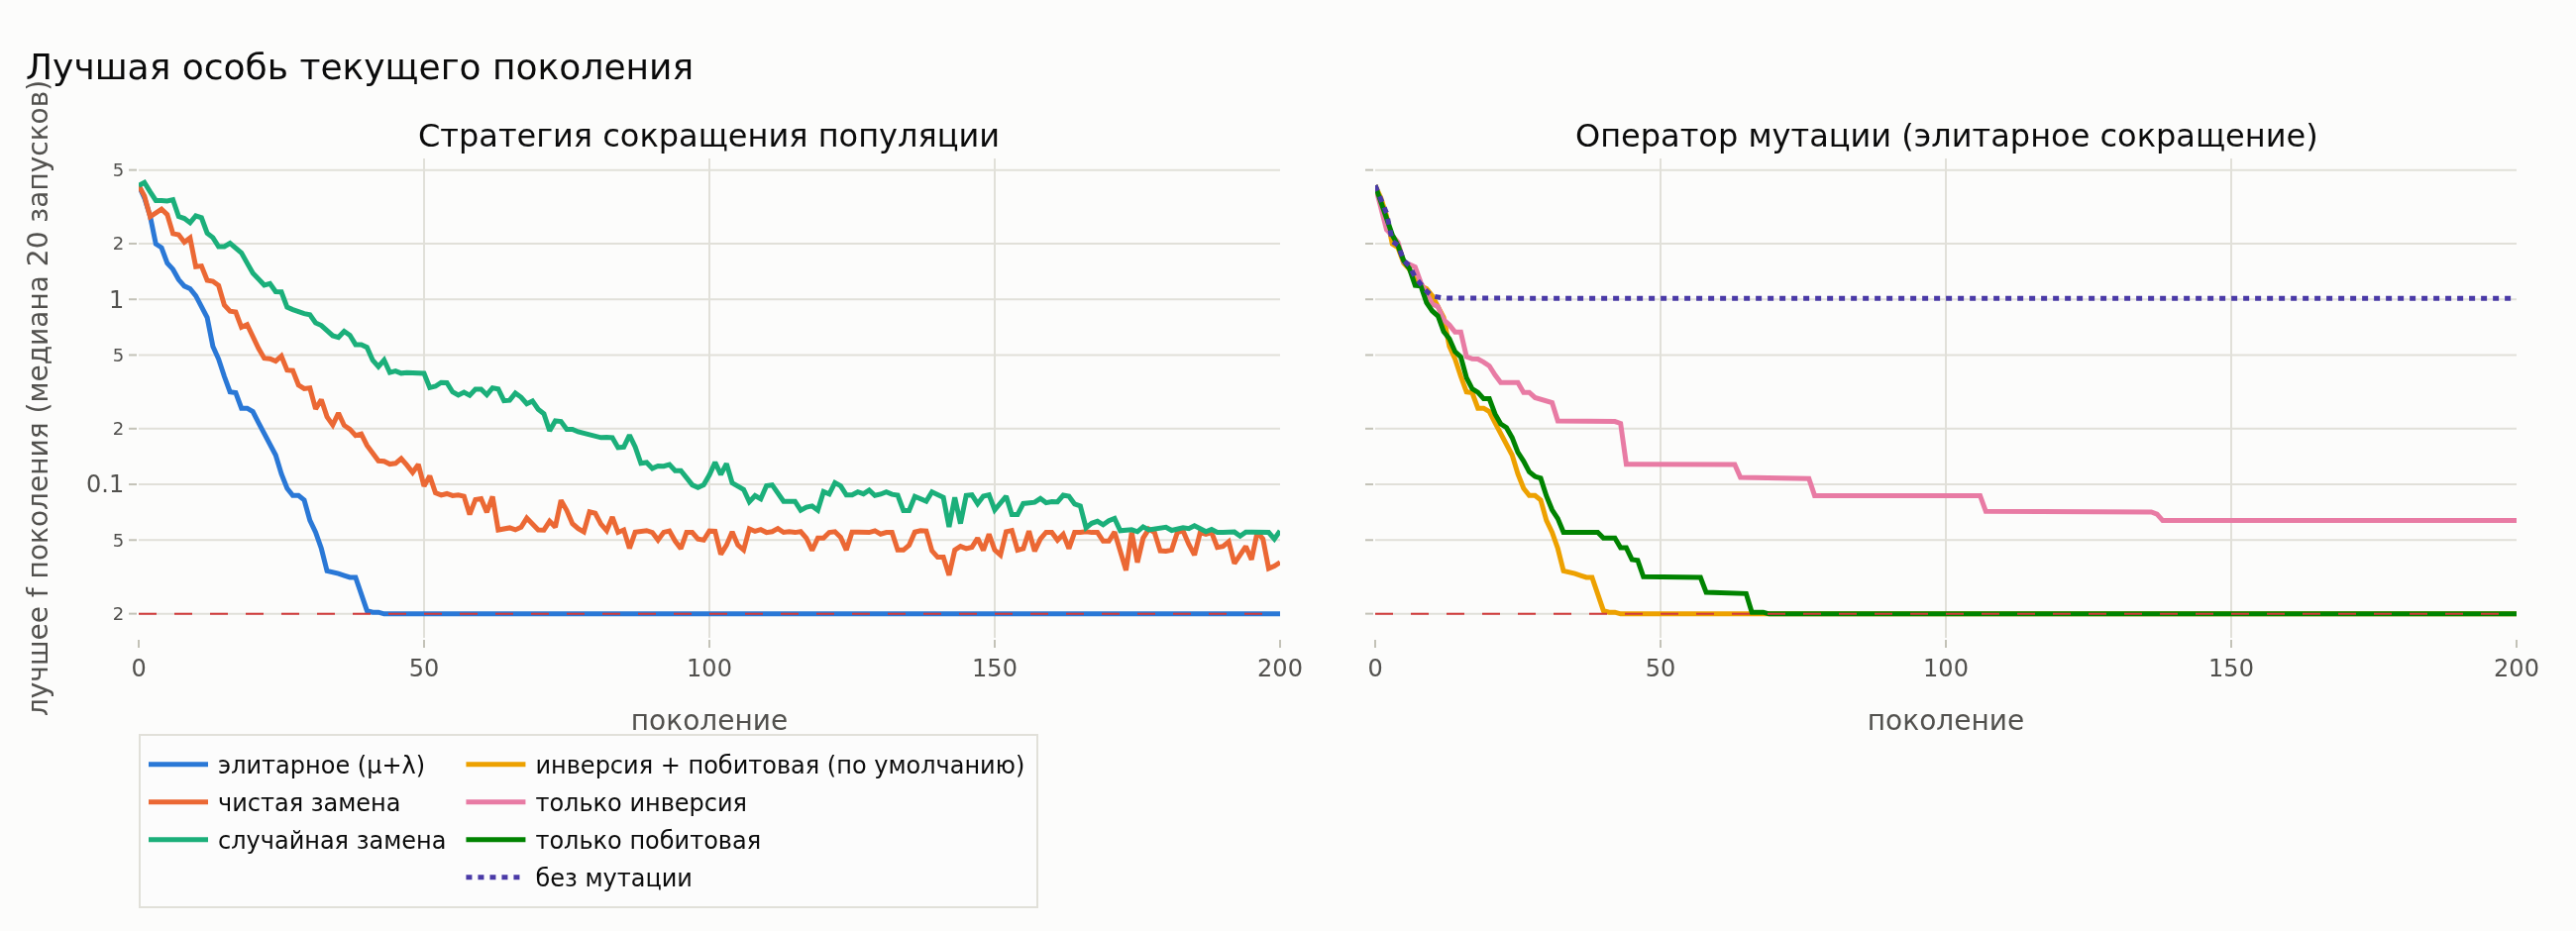
\includegraphics[width=\textwidth]{04_reduction_mutation.png}
\caption{Лучшая особь текущего поколения (медиана 20 запусков): стратегии сокращения и операторы мутации}
\label{fig:red}
\end{figure}

\textbf{Параметры.} Влияние размера популяции, вероятностей кроссинговера и инверсии и размера турнира~--- в таблице~\ref{tab:params} и на рисунке~\ref{fig:params}.

\begin{figure}[H]
\centering
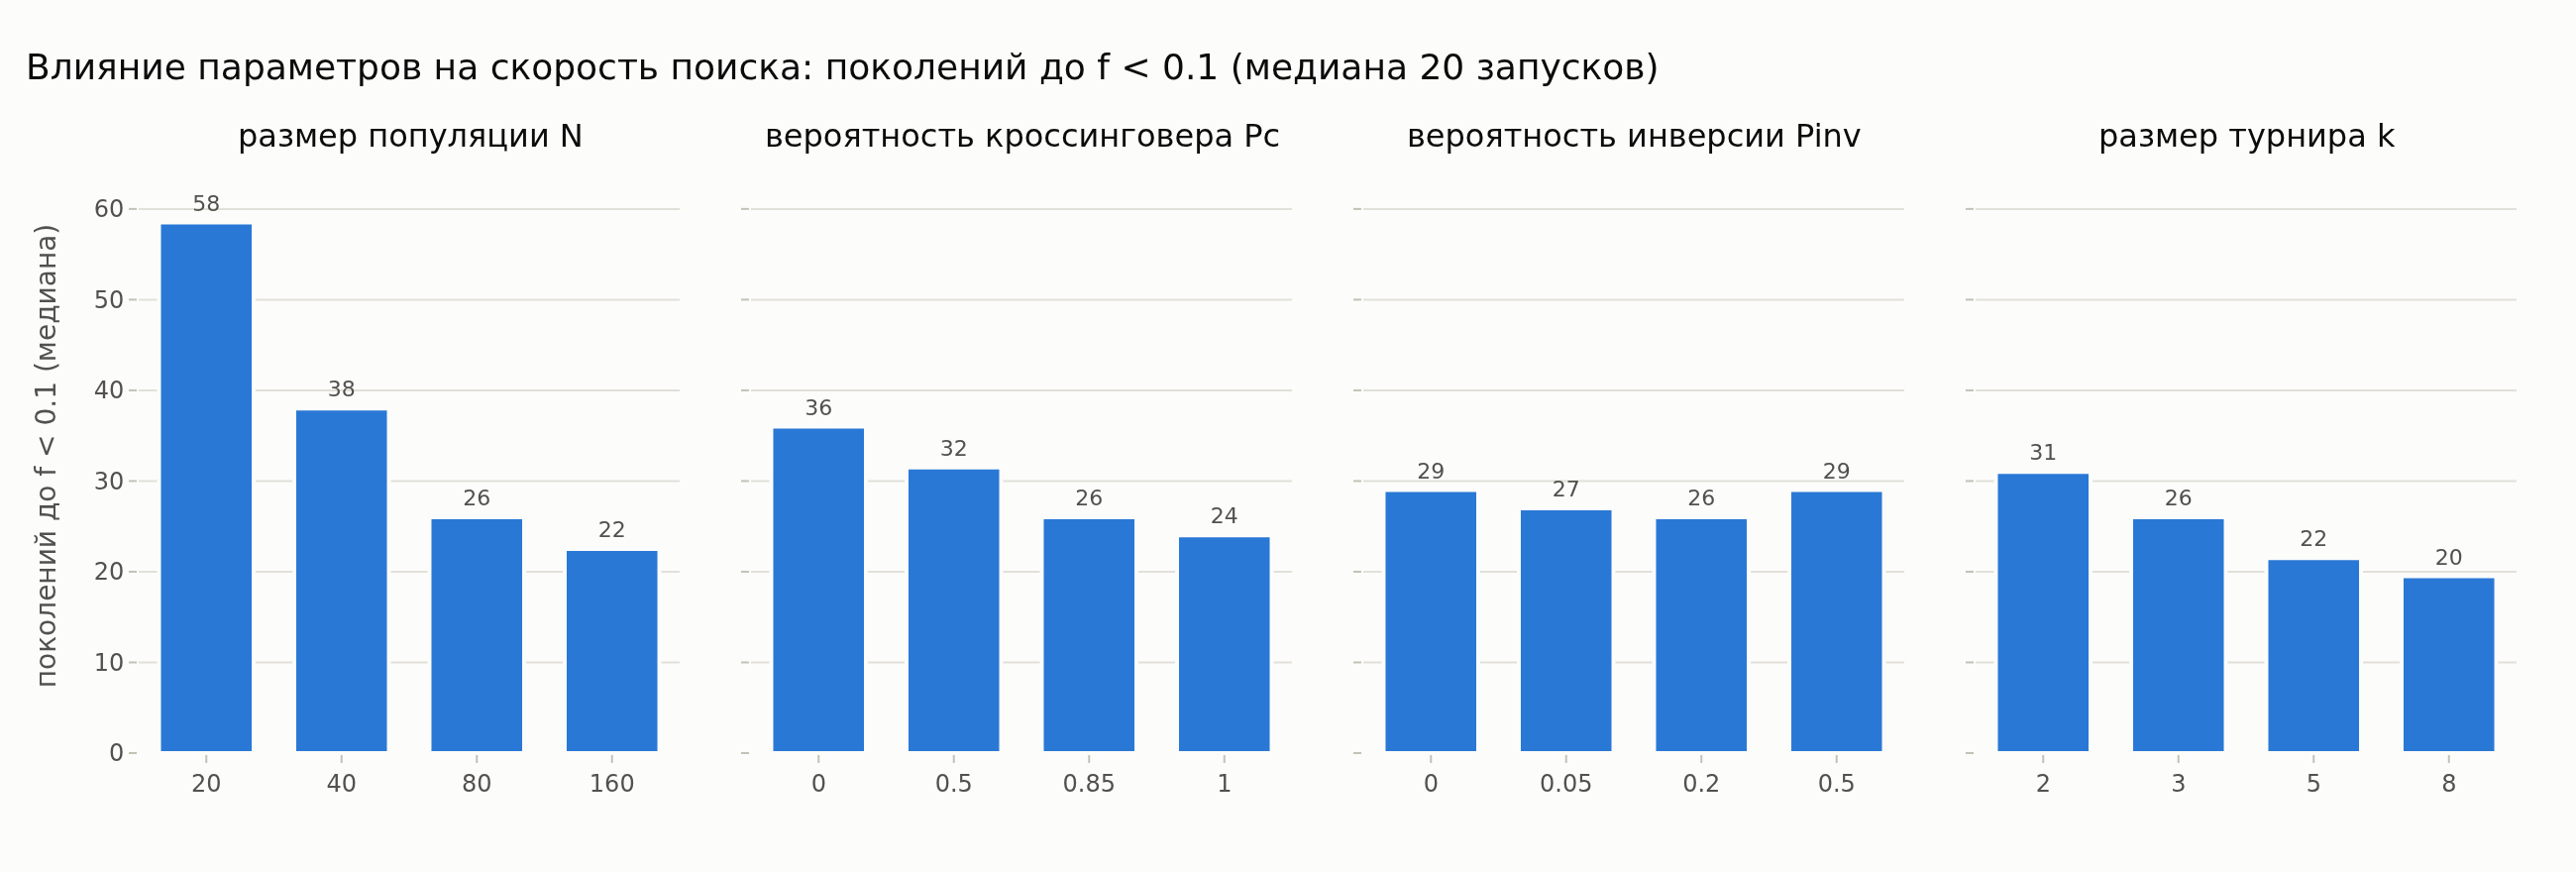
\includegraphics[width=\textwidth]{05_parameters.png}
\caption{Скорость поиска: число поколений до $f < 0{,}1$ (медиана 20 запусков)}
\label{fig:params}
\end{figure}

\begin{table}[H]
\caption{Влияние параметров ГА (20 запусков на значение)}
\label{tab:params}
\centering
\small
\begin{tabular}{lccccc}
\toprule
Параметр & Значение & Худшее $f$ & Успехов, \% & До предела, \% & Поколений \\
\midrule
размер популяции N & 20 & 0.240 & 80 & 70 & 58 \\
размер популяции N & 40 & 0.087 & 100 & 70 & 38 \\
размер популяции N & 80 & 0.031 & 100 & 90 & 26 \\
размер популяции N & 160 & 0.020 & 100 & 100 & 22 \\
вероятность кроссинговера $P_c$ & 0 & 0.055 & 100 & 80 & 36 \\
вероятность кроссинговера $P_c$ & 0.5 & 0.031 & 100 & 85 & 32 \\
вероятность кроссинговера $P_c$ & 0.85 & 0.031 & 100 & 90 & 26 \\
вероятность кроссинговера $P_c$ & 1 & 0.031 & 100 & 85 & 24 \\
вероятность инверсии $P_{inv}$ & 0 & 0.055 & 100 & 80 & 29 \\
вероятность инверсии $P_{inv}$ & 0.05 & 0.031 & 100 & 95 & 27 \\
вероятность инверсии $P_{inv}$ & 0.2 & 0.031 & 100 & 90 & 26 \\
вероятность инверсии $P_{inv}$ & 0.5 & 0.087 & 100 & 95 & 29 \\
размер турнира k & 2 & 0.020 & 100 & 100 & 31 \\
размер турнира k & 3 & 0.031 & 100 & 90 & 26 \\
размер турнира k & 5 & 0.032 & 100 & 80 & 22 \\
размер турнира k & 8 & 0.035 & 100 & 90 & 20 \\
\bottomrule
\end{tabular}
\end{table}


\section{Выводы}

\begin{enumerate}
\item ГА находит точку $(-1{,}0 \cdot 10^{-4};\ 1{,}0 \cdot 10^{-4})$ с $f = 0{,}0200$~--- точный предел 20-битного кода. За 10 поколений популяция стягивается с области $\pm 100$ к кольцам радиусом несколько единиц; медианный запуск достигает предела к 40-му поколению.
\item В 20 запусках успех~--- 100\,\%, предел сетки достигнут в 90\,\% запусков, медиана~--- 26 поколений до $f < 0{,}1$.
\item Инверсия без побитовой мутации слаба: 70\,\% успехов и лишь 10\,\% запусков до предела. Она только переставляет биты и не создаёт недостающих значений. Вместе с побитовой мутацией~--- 100\,\% успехов, 90\,\% до предела и лучшее худшее значение ($0{,}031$). Без мутации популяция вырождается (5\,\% успехов).
\item Стратегия сокращения определяет скорость: элитарная~--- 26 поколений и 90\,\% до предела, чистая замена~--- 44 и 65\,\%, случайная~--- 84 и 35\,\%. Без элитизма лучшие особи теряются.
\item Рост популяции с 20 до 160 ускоряет поиск (58 $\to$ 22 поколения) и поднимает долю запусков до предела с 70 до 100\,\%. Больший турнир ускоряет сходимость (31 $\to$ 20 поколений при $k = 2 \to 8$), кроссинговер~--- тоже (36 $\to$ 24 при $P_c = 0 \to 1$).
\end{enumerate}


\end{document}
